\documentclass[12pt]{article}
\usepackage{graphicx} % For including graphics
\usepackage{hyperref} % For URLs and hyperlinks
\usepackage{amsmath} % For math symbols
\usepackage{enumitem} % For customized lists
\usepackage{geometry} % For page margins
\usepackage{xcolor} % For colored text
\usepackage{titlesec} % For title formatting
\usepackage{fancyhdr} % For headers
\usepackage{setspace} % For spacing
\usepackage{multirow}
\usepackage{adjustbox} % For scaling the table
\usepackage{array} % For defining column widths and centering
\usepackage{float}
\usepackage{rotating} % For sideways tables
\usepackage{tabularx} % For automatically adjusting column widths
\usepackage{placeins} % For \FloatBarrier
\usepackage{caption}
\usepackage{subcaption}
\usepackage{longtable}
\usepackage{lscape}
\usepackage{booktabs}

% Page setup
\geometry{a4paper, margin=0.75in}
\setlength{\parindent}{0pt} % Remove indentation
\captionsetup{font=scriptsize}

% Header setup
\pagestyle{fancy}
\fancyhf{}
\fancyhead[L]{Group No: C1}
\fancyhead[C]{ME 407 -- Spring 2024}
\fancyhead[R]{\thepage}
\renewcommand{\headrulewidth}{0.4pt}

% Document Title
\begin{document}
\begin{center}
    \vspace{1em}
    \textbf{\LARGE PROBLEM DEFINITION AND DESIGN\\ \vspace{8pt}SPECIFICATIONS}\\
    \vspace{1em}
    \textbf{PROJECT: Design of an Automatic Table Tennis Ball Pitcher}
\end{center}

\section{Definition of the Problem}
Table tennis is a sport that keeps rising in popularity day by day, as it can be easily enjoyed by all age groups, and the rules are easy to pick up. Aside from being an Olympic sport, it is also widely played as a hobby by a large number of people, and some studies even suggest that for children and the elderly, the sport has various physical and mental health benefits. Taking these into consideration, it can be seen in Figure \ref{fig:wholesales} that the demand for the sport is increasing each year.

\begin{figure}[H]
    \centering
    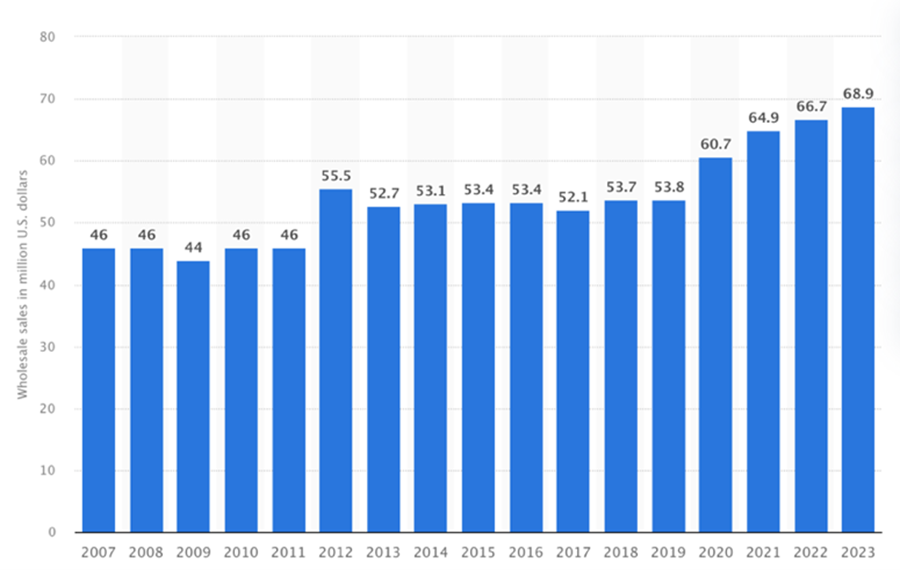
\includegraphics[width=0.6\textwidth]{figures/wholesales.png}
    \caption{Table tennis equipment wholesale sales in the U.S. from 2007 to 2023 (in million U.S. dollars) \cite{statista2024}}
    \label{fig:wholesales}
\end{figure}

For such a popular sport that spans from a professional and competitive scene to leisure time hobby for a large demographic, a prominent issue may be expressed as its requirement of two people to be played. A willing partner to practice with may not be readily available at all times, and this poses a problem for both professional players who need to practice and hone their skills for competition, and the general population who seek to play it for various reasons ranging from pastime hobby to a healthy lifestyle. For this reason, the need for a product that allows people to practice the sport on their own is apparent. However, the already existent products on the market are either too expensive to serve a broader customer population or lack some features that may result in a poorer experience. This project aims to fill the gap and create a table tennis ball pitching machine suitable for players of all skill levels, from amateur to professional. \\

To accomplish this goal, the machine should be adjustable from an easy operational mode to more complex and harder-to-predict operations to imitate a real person as closely as possible. It should be able to perform simple and basic pitches, as well as adjust to give the ball various spin options, pitch the ball at different locations, pitch at varying speeds and frequencies, and switch between these variations automatically. Additionally, a mechanism should be implemented to ensure the machine can recycle the returned balls to self-supply for longer and more continuous operation, allowing for uninterrupted and more efficient play time.
\quad 

\section{Project Requirements}
\begin{itemize}
    \item The design should feature an adjustable serving frequency, allowing for a varying number of balls per minute.
    \item The serving speed should be adjustable, with automatic adjustment preferred, ranging from low to high velocity.
    \item Balls should land on the side of the table across the net for normal shots.
    \item The machine should be able to throw the ball back from the net and have it bounce once on each side (optional feature).
    \item Serving angles should be automatically adjustable within a specified range of degrees.
    \item The horizontal position on the table from which balls are launched should be manually adjustable.
    \item The design should have a large enough capacity to contain a sufficient number of balls.
    \item The design should be lightweight, ensuring it can be carried and assembled by a single person.
    \item Balls returned from within a defined area on the table and up to a certain height should be recyclable into the system.
    \item The system should be compatible with standard table tennis tables, as defined by the ITTF.
    \item The design should accommodate standard table tennis balls.
    \item The machine should be able to launch balls with no spin.
    \item The system should have a user-friendly interface for adjusting serving speed, angle, spin, and frequency.
    \item The machine should operate on standard mains electricity
\end{itemize}
\quad 
\section{Design Specifications}
\begin{itemize}
    \item The design should have serving frequency range that 25-80 balls per minute. It can easily reach the maximum serving frequency value.
    \item The design should have adjustable serving speed range in between 4 m/s to 25 m/s.
    \item It should allow uninterrupted training with desired
    frequency.
    \item A minimum of 7 serving points on the table, including both sides, as seen in Figure \ref{fig:7areaoftable}.
    \begin{figure}[H]
        \centering
        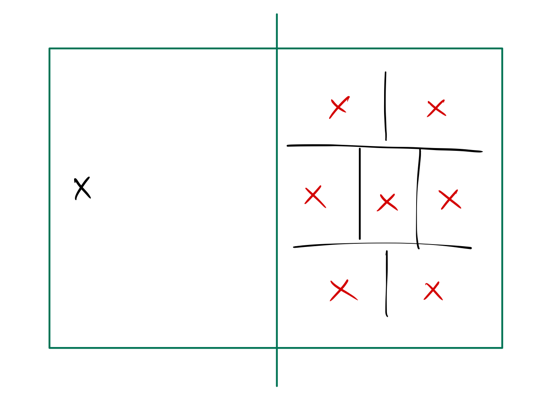
\includegraphics[width=0.4\textwidth]{figures/7areaoftable.png}
        \caption{Table Tennis Serving Points on Table}
        \label{fig:7areaoftable}
    \end{figure}
    \item The thrown balls should hit the 7 serving points within the 5 cm radius range.
    \item The design can be controlled and adjusted easily.
    \item Pitch angle should be adjustable within -20 to +20 degrees.
    \item Yaw angle should be adjustable within -20 to +20 degrees.
    \item Minimum storage capacity of 100 balls.
    \item Maximum weight of 15 kg for portability.
    \item The design can collect the properly returned balls from the player. Recyclable ball height needs to be at least 1 meter.
    \item The design needs to fit standard table tennis tables where standard table dimensions 2.74 m x 1.525 m.
    \item The machine should serve over a net height of 15.25 cm.
    \item Ball specifications: 40 mm diameter, 2.7 g weight.
    \item Lifetime of a single ball in the cycle should be at least 1000 throws.
    \item The design should ensure spin capability that can give 36 different spins (top spin, back spin, side spins).
    \item The design when un-assembled should fit inside a $1m^3$ box.
    \item The machine should operate on standard mains electricity (220-240V, 50-60 Hz). Also, it should not consume too much power that is not necessary.
    
\end{itemize}
\quad 
\section{Design Criteria}
\begin{enumerate}
    \item Maximum Attainable Serving Frequency (12\%): Can throw 80 balls per minute and more.
    \item Adjustment Accuracy of Serving Frequency (12\%): Adjustable within 25-80 balls per minute.
    \item Automatic Feeding at Certain Frequency: Allows for uninterrupted training with desired frequency.
    \item Collecting Properly Returned Balls into the reservoir: The design can collect balls that came up to 1 meter height on its side.
    \item Serving Accuracy and Precision (6\%): Balls must hit the 7 serving points within 5 cm radius range.
    \item Maximum Attainable Serving Speed (15\%): Adjustable between 4 m/s and 25 m/s. Can throw balls at 25 m/s and more.
    \item Selectable Serving Modes (10\%): Supports various training modes.
    \item Adjustment Accuracy of Pitch and Yaw Angle (10\%): Angles adjustable within specified ranges accurately.
    \item Ease of control: The design can be controlled and adjusted easily.
    \item Portability (8\%): Maximum weight 15 kg, easy to set up.
    \item Capacity (5\%): Minimum storage of 100 balls.
    \item Ball Durability (5\%): Balls should withstand at least 1000 throws.
    \item Power Consumption (3\%): Energy efficiency prioritized.
    \item Spin Options (10\%): Ability to generate 36 spins for varied training.
    \item Cost (4\%): Adjustable settings for ball trajectory, speed, and spin.
    \item Ease of manufacture: The design should not be too difficult to produce. It should not contain complicated elements.
    \item No Spin (Bonus 5\%): Optional feature to throw without spin.
    \item Special Serving (Bonus 5\%): Optional feature for specific serving modes.
\end{enumerate}
\quad 

% References section
\bibliographystyle{IEEEtran} % or any style you prefer
\bibliography{bibliography}

\end{document}
